% !Mode:: "TeX:UTF-8"   %%winedt 以utf8编码打开
% Can only be compiled with xelatex+bibtex

%双行标题
% \documentclass[twoside,longtitle]{LZUthesis}
%单行标题
\documentclass[twoside]{LZUthesis}

\usepackage{float}
\usepackage{fancybox}
\usepackage{calc}
% \usepackage{mathdots}
\usepackage{graphicx}
\usepackage{listings}

%声明图片后缀名
\DeclareGraphicsExtensions{.pdf,.eps}

\makeatletter

% 设置图形文件的搜索路径
\graphicspath{{figures/}}

% 小节标题靠左对齐
\CTEXsetup[format+={\flushleft}]{section}

% 取消链接的颜色(黑白打印时启用)
%\hypersetup{colorlinks=false}

%使文档居中,打印时应注释掉
%\evensidemargin 0.93 true cm
\setlength{\hoffset}{-0.3 cm}

%允许equationarray分页换行
\allowdisplaybreaks

%使字体清晰,且透明位图不会使页面文字粗细不一
\usepackage{eso-pic}
\AddToShipoutPicture{%
\special{pdf: put @thispage <</Group << /S /Transparency /I true /CS /DeviceRGB>> >>}%
}

%页面背景色
%\definecolor{yellow}{rgb}{0.99,0.99,0.70}
%\pagecolor{yellow}

%浮动项超链接正确跳转
\usepackage[all]{hypcap}

\makeatother


\begin{document}

%分类号;一般不要求学生填写
\classification{}

%密级;申请保密后需填写
\confidential{}

%中文标题
\title{铁磁石墨烯中近藤效应的数值重整化群研究}

%中文标题第二行,题目较短时删除之,并去除文档类选项 longtitle
% \titleadd{\LaTeX{}模板简介}

%英文标题
\englishtitle{}

%英文题目第二行,题目较短时删除之,并去除文档类选项 longtitle
% \englishtitleadd{Lanzhou University Thesis}

%作者汉语姓名
\author{李高阳}

%专业
\major{物理学$\cdot$理论物理}

%学位
\degree{博士}

%研究方向
\direction{凝聚态理论}

%导师姓名+职称
\advisor{罗洪刚~教授~~~~~~房铁峰~教授}

%论文工作起止年月
\datebeginAndEnd{2015年9月至2019年6月}

%论文提交日期
\submitdate{}

%答辩日期
\defenddate{}

%学位授予日期
\degreedate{}

%左侧页眉
\lzuthesis{兰州大学博士学位论文}

%生成封面
\maketitle

%生成声明页
\makestatement

%前文-罗马页码
\frontmatter\pagenumbering{Roman}

%中文摘要
\begin{abstract}
\end{abstract}

%中文关键词
\keywords{}

%英文摘要
\begin{englishabstract}
\end{englishabstract}

%英文关键词
\englishkeywords{}

%自动生成章节目录以及pdf书签
\tableofcontents{}


%正文部分-数字页码
\mainmatter

%正文页眉页脚样式
\pagestyle{lzu}

\chapter{引言\label{chap:intro}}
简述量子多体问题,引出量子杂质问题
\section{量子杂质问题}
量子杂质问题描述的是一个多体相互作用(通常为库仑相互作用或交换相互作用)发生在单个位点(杂质)上的系统,并且杂质与一个由宏观数量的无相互作用粒子组成的热库相互作用。
\begin{figure}[!hb]
\centering
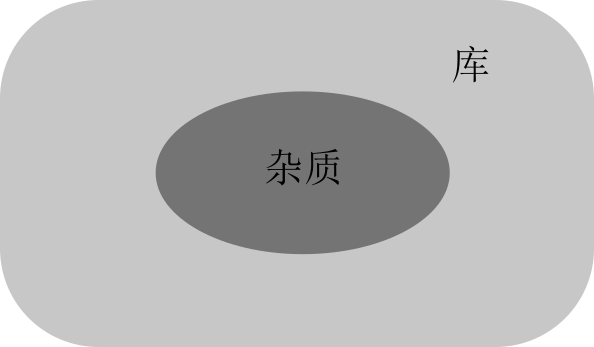
\includegraphics[width=0.5\textwidth]{QIM.png}
\caption{量子杂质模型的示意图。系统包括了三部分:杂质部分、库、杂质与库的耦合。}
\end{figure}
热库的粒子可以是玻色子(声子、磁振子、粒子-空穴对等)也可以是费米子(导带电子等),杂质可以是真实的杂质(如在金Au中掺杂的铁Fe原子,在石墨烯上吸附的钴Co原子),也可能是与电磁场相作用的二能级原子,或表现为量子点的一块小的受限区域等。它们可以用近藤模型、安德森模型、自旋玻色模型等来描述,一般地表示为 $H = H_{\rm{imp}} + H_{\rm{bath}} + H_{\rm{hyb}}$, $H_{\rm{imp}}$ 为杂质电子哈密顿量,$H_{\rm{bath}}$ 表示库电子哈密顿量,$H_{\rm{hyb}}$ 表示杂质电子与库电子的耦合。
本文以单杂质安德森模型为例进行说明,对于单杂质安德森模型:
\[
H_{\rm{imp}} = \sum_{\sigma} \varepsilon_{d\sigma}d^{\dag}_{\sigma}d_{\sigma} + Un_{d\uparrow}n_{d\downarrow},
\]
\[
H_{\rm{bath}} = \sum_{k\sigma}\varepsilon_{k\sigma}c^{\dag}_{k\sigma}c_{k\sigma},
\]
\[
H_{\rm{hyb}} = \sum_{k\sigma}(V_{k\sigma}c^{\dag}_{k\sigma}d_{k\sigma} + H.c.).
\]
其中,$d^{\dag}_{\sigma}(d_{\sigma})$为杂质电子的产生(湮灭)算符,$\varepsilon_{d\sigma}$表示杂质$d$电子自旋依赖的能级位置,$\sigma$为系统的自旋指标,取值为$\uparrow$或$\downarrow$,$n_{d\sigma}=d^{\dag}_{\sigma}d_{\sigma}$为杂质电子的粒子数算符,$U$为杂质能级被又占据时的为库仑排斥能。$c^{\dag}_{k\sigma}(c_{k\sigma})$算符产生(湮灭)一个动量为$k$,自旋为$\sigma$的库电子,$\varepsilon_{k\sigma}$为库电子的色散关系。最后一项哈密顿量$H_{\rm{hyb}}$描述了杂质电子与库电子的耦合,耦合强度为$V_{kd}$。
\section{量子点系统中的近藤效应}
\subsection{量子点}
\subsection{近藤效应}
\subsection{与正常电极连接的量子点}
\subsection{与铁磁电极连接的量子点}
\section{石墨烯中近藤效应}
\subsection{赝能隙Anderson模型}

\chapter{全密度矩阵数值重整化群(FDM-NRG)}

\chapter{石墨烯中铁磁增强的近藤效应}


\chapter{受门电压调控的铁磁性石墨烯中的近藤效应}


\chapter{总结与展望}

\section{总结}
\section{展望}


\bibliographystyle{lzubib}
\bibliography{bib/thesis}
%\bibliographystyle{revtex4-1}
%\bibliography{bib/thesis}
\iffalse
\renewcommand{\baselinestretch}{1}\zihao{5}\begingroup\raggedright\begin{thebibliography}{100} \makeatletter
	\bibitem{Jandl1996_7318}
	S.~Jandl, M.~Poirier, M.~Castonguay, P.~Fronzes, J.~L. Musfeldt,
	A.~Revcolevschi, and G.~Dhalenne.
	{\it Phonons in pure and doped ${\mathrm{CuGeO}}_{3}$ spin-peierls crystals: Raman and ultrasonic studies}.
	\href{https://link.aps.org/doi/10.1103/PhysRevB.54.7318} {Phys.	Rev. B \textbf{54}, 7318 (1996)}.

\end{thebibliography}
\fi

%发表文章目录
\begin{publications}{99}
\item[]  \textbf{发表的论文:}
\item \textbf{Bin-Bin Mao(毛斌斌)}, Maoxin Liu(刘卯鑫), Wei Wu(吴威), Liangsheng Li(李粮生), Zu-Jian Ying(应祖建), Hong-Gang Luo(罗洪刚), \textit{An analytical variational method for the biased quantum Rabi model in the ultra-strong coupling regime}, \href{http://iopscience.iop.org/article/10.1088/1674-1056/27/5/054219}{Chin. Phys. B, 2018, 27:054219}.

\item[]  \textbf{参与的项目:}
\item[$1.$]自然科学杰出青年基金(11325417):凝聚态理论与数值方法。
\item[$2.$]自然科学面上基金(11174115):少电子系统中电子关联的大尺度计算研究。
\item[$3.$]自然科学面上基金(11674139):量子杂质系统中的新奇量子态研究。
\item[$4.$]教育部创新团队基金(IRT1251,IRT16R35)。

\end{publications}


\chapter{致谢}

\begin{thanks}

\end{thanks}

\end{document}
